%!TEX root = ../thesis.tex
%*******************************************************************************
%****************************** Second Chapter *********************************
%*******************************************************************************

\chapter{General physical properties of 2D materials \label{chap:3}}

\ifpdf
    \graphicspath{{Chapter3/Figs/Raster/}{Chapter3/Figs/PDF/}{Chapter3/Figs/}{Chapter3/Figs/Vector/}}
\else
    \graphicspath{{Chapter3/Figs/Vector/}{Chapter3/Figs/}}
\fi

In this thesis, the properties of materials are divided into a preliminary and an advanced category, where the latter will be presented in the next chapter as the main results of this thesis. In this chapter, I will focus on the preliminary properties of 2D materials, namely structural, electronic, vibrational and mechanical properties. These properties can be used to test the methodology and form the foundation upon which the advanced properties are calculated. They are composed both of my original calculations and results from literature. An emphasis will be on the characteristic properties of 2D materials that are different from 3D materials.

\section{Structural properties}
\subsection{Layered structure: from multi- to monolayer}

As discussed in \autoref{chap:1}, layered bulk materials are closely related to 2D materials. A single layer of a layered bulk material is a 2D material. This anisotropic nature is attributed to the weak interlayer bonds and the strong intralayer bonds. Van der Waals (vdW) interaction \cite{vdws} is the main source of the weak interlayer bonds. vdW interactions consist of the attraction and the repulsion between atomic or molecular entities caused by dipole-dipole, dipole-induced dipole and instantaneous induced dipole-induced dipole forces. The definition is sometimes extended to include all dispersion forces between molecules.  For 2D materials, the vdW interaction becomes important as the number of layers is larger than one; that is few-layer materials having typically less than ten layers. They also belong to the family of 2D materials since the thickness of the materials is still small and quantum confinement effects are very important. As in its layered bulk counterpart, a few-layer system is a stack of monolayers hold together through vdW forces. When no other bonding types are present, interlayer vdW interaction determines all the change when going from a single layer to multi-layer, and its impact on the electronic structure can be significant. For example, from monolayer to bilayer, the low energy linear dispersion relation of energy $E$ as a function of $k$ around the $\mathrm{K}$ point evolves into a parabolic-like spectrum\cite{Partoens2006,Mak2010a}. 

\begin{figure}[ht] 
\centering  
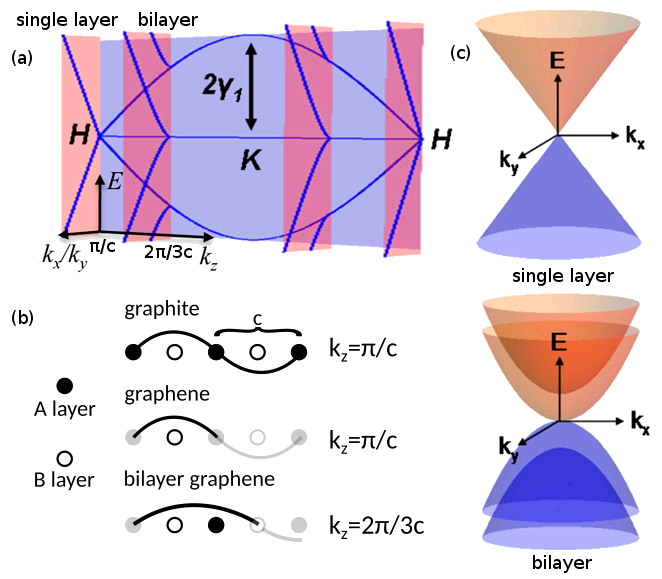
\includegraphics[width=0.9\textwidth]{gra_band.png}
\caption{(a) Energy-momentum dispersion relations of single layer and bilayer graphene as approximated by plane intersections of 3D graphite dispersion relation and (b) their 3D dispersion relations around the $\mathrm{K}$ point. (c) Matching of the wavelength in graphite to that in single layer and bilayer graphene. Image is adapted from Ref. \cite{Mak2010a}. }  
\label{fig:gra_bands}
\end{figure} 

In \autoref{fig:gra_bands} (a), the dispersion relation of graphite along the z direction, that is the HKH line in the Brillouin zone, is shown on the blue plane. This direction is perpendicular to the graphite layers. Because of quantum confinement in a few-layer system,  standing waves are presented with a finite number of wave vectors.  If only the intralayer and interlayer interactions between the nearest neighbour atoms were considered, the dispersion relation in few-layer graphene can be approximated as those on the cross-section of virtual planes (the red planes in \autoref{fig:gra_bands} (a)) with the 3D graphite dispersion relation.  These planes are perpendicular to the z direction and intersect with the HKH line at limited points. This is called the quantization\footnotemark\footnotetext{Sometimes it is also referred as zone-folding.} of dispersion relations\cite{saito1998physical}. These points are illustrated in \autoref{fig:gra_bands} (c). Quantum confinement in a few-layer system requires that the wave functions vanish at the imaginary layer right outside the surface of the system, the systems will have well-defined wave vectors. Then, the dispersion relations of graphene and bilayer graphene will be on the red planes that intersect the HKH line at $k_z=\pi/c$ and at $kz=2(\pi/3c)$, respectively, where $c$ is the lattice constant of graphite that is vertical to the graphite plane.  Having the knowledge of the 3D band structure of graphite, one can approximate the dispersion relation of few-layer systems in this way. As shown in the red plane in \autoref{fig:gra_bands} (a) and the 3D version in \autoref{fig:gra_bands} (b), graphene has a linear dispersion relation and bilayer graphene has two parabolic-like bands. Moreover, the bilayer structure will never pass through the H point where graphene has passed to have a linear dispersion relation. This is because the standing waves in a bilayer will have a wave vector $k=2(n \pi/3c)$, where $n$ is a positive integer: 1, 2, ... , n. This will never be equal to $\pi/c$ for any integer number of $n$. More generally, systems with an even number of layers will not have a linear dispersion relation, and vice versa for systems that have an odd number of layers. Further, if other interactions were considered, an overlap of those bands touching each other would have occurred\cite{Partoens2006}. This overlap increases with the number of layers. Eventually, maximum overlap is reached in graphite.


\begin{figure}[htbp!] 
\centering  
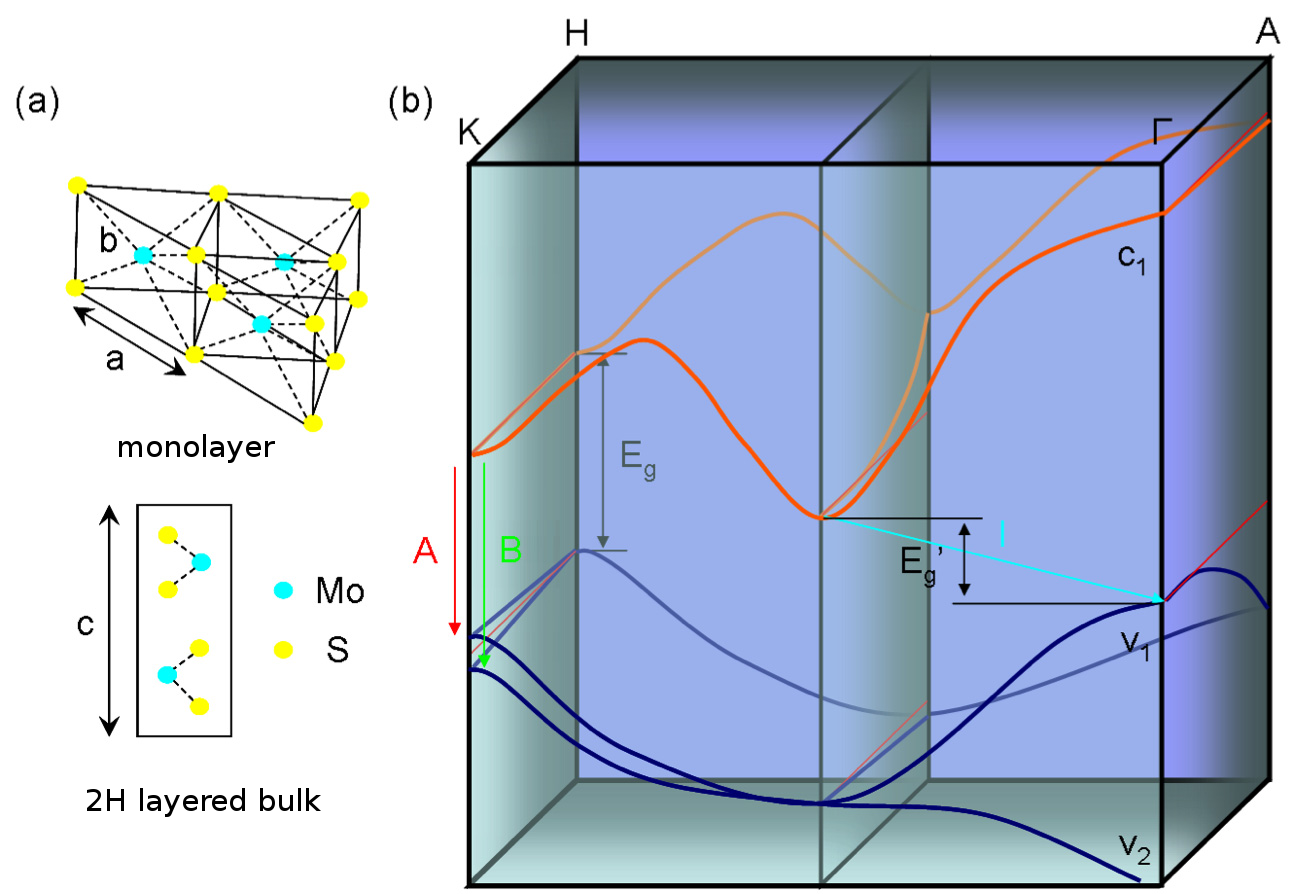
\includegraphics[width=0.8\textwidth]{mos2_band.png}
\caption{(a) The atomic structures of monolayer and layered bulk MoS$_2$. (b) The energy-momentum dispersion relation of monolayer MoS$_2$ as a plane intersection of the 3D dispersion relation. Image is adapted from Ref. \cite{Mak2010}. }  
\label{fig:mos2_band}
\end{figure} 

Another example of the importance of interlayer interactions in few-layer 2D materials is seen for MoS$_2$. As mentioned in \autoref{chap:1}, as going from layered bulk to monolayer, MoS$_2$ transforms from an indirect band gap to a direct one. Here again, we can make use of the quantization scheme to approximate the band structure of the monolayer from that of its layered bulk. The monolayer and the layered bulk structure of the 2H phase are shown in \autoref{fig:mos2_band} (a). In \autoref{fig:mos2_band} (b), let us focus on the planes parallel to the page that pass through the $\mathrm{K}\Gamma$ line and the HA line (simply call them $\mathrm{K}\Gamma$ plane and HA plane below). Similar to the previously discussed graphite, 2H layered bulk MoS$_2$ has two layers per unit cell. Therefore, according to the standing wave arguments that we have used for the graphene case above, HA plane represents the monolayer. $E_g$ and $E\prime_g$ are the band gaps of the monolayer and the layered bulk structures. Here, not only the magnitude of the band gap is increased as going from layered bulk to monolayer, the character of the band gap has changed as well. It is clearly shown that this is due to the shifting of the band edges. VBM at $\Gamma$ and CBM at the middle of the $\Gamma\mathrm{K}$ line are brought closer as they go from monolayer to layered bulk. This corresponds to the widening of the band width and it is coming from the splitting of the VB and CB when more and more layers interact with each other through the interlayer interactions. Therefore, the band gap in the layered bulk is defined by these two band edges, which in the monolayer was defined by the band edges at $\mathrm{K}$. In contrast to this, the band edges at the $\mathrm{K}$ point are not affected too much by the interlayer interaction. So why do the band edges react differently to the interlayer interactions? If we look into the orbital composition of the band edges, we will find the ones that have widened the most, i.e. VBM at $\Gamma$, have the largest contribution from S $p_z$ and Mo $d_{z^2}$ orbitals. These out-of-plane orbitals are orientated vertically to the plane and thus have maximum overlap with the others from an adjacent layer. Therefore, band splitting is more profound for these band edges and causing the increase of their band width. In contrast, both the CBM and VBM at $\mathrm{K}$ are largely composed of S $p_x$ and $p_y$ orbitals and Mo $d_{xy}$ and $d_{x^2-y^2}$ orbitals. All of them are in-plane orientated orbitals and thus have limited effect from the interlayer interaction\cite{Padilha2014}.

\subsection{sp$^n$ hybridization\label{sphyb}}

After discussing layered structures and the importance of interlayer interaction, let us look into some detail of the in-plane structure and how sp$^n$ hybridization gives rise to various structures for 2D materials, where $n$ is the hybridization index that will be discuss in the following. When atoms come together to form bonds, the orientation of bonding orbitals are decisive for the final structure. The hybridization of s and p orbitals is a good example of this.  It mainly exists in three different variants: sp, sp$^2$ and sp$^3$, see \autoref{fig:sp_hybrid}. The hybridization index $n$ in sp$^n$ stands for the relative amount of p character in the resulting hybridized orbital. For example, sp$^2$ has 1/3 s character and 2/3 p character. Hybridized orbitals tend to maximize their distance to reduce the energy raised by the repulsion of electrons. As shown in \autoref{fig:sp_hybrid}, this results in tetrahedral structure of sp$^3$ orbitals, as in diamond, trigonal planar structure of sp$^2$ orbitals, as in graphene or graphite and linear structure of sp orbitals, as in ethyne molecules.  This is, for example, useful to explain the buckled structure of graphane and fluorographene. Because sp$^3$ character is induced when the fourth electron is bonded with H or F atoms, and as a result buckling appears in these systems. 

\begin{figure}[htb] 
\centering  
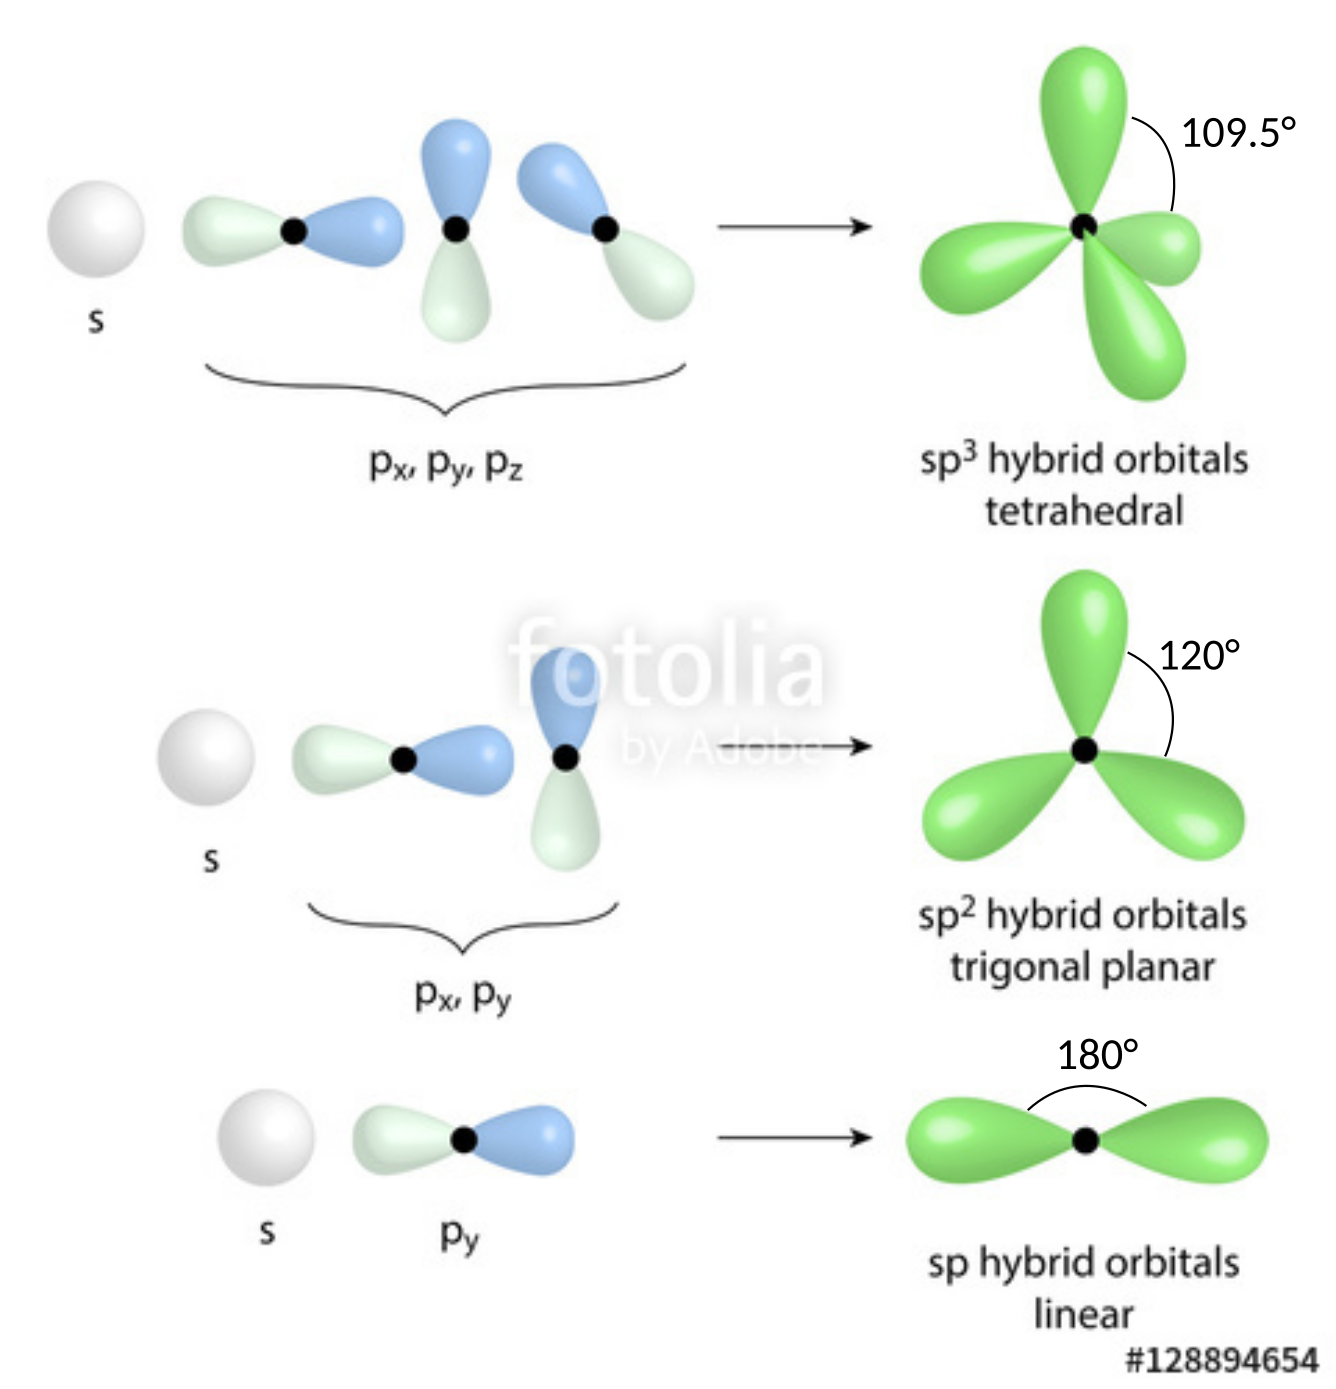
\includegraphics[width=0.8\textwidth]{sp_hybrid.png}
\caption{Three types of sp hybridized orbitals. Image is adapted from Ref. \cite{sp_hybrid}. }  
\label{fig:sp_hybrid}
\end{figure} 

\citet{coulson1949} generalized the relation of bond angle with $n$ as follows:
\begin{equation}\label{coulson}
1=-\sqrt{n_1n_2}~cos\theta_{12}, 
\end{equation}
where $\theta_{12}$ is the bond angle between orbital 1 and 2. If orbital 1 and 2 have different $n_1$ and $n_2$, we still need one more constraint to solve the \autoref{coulson} for the hybridization indices $n$. This constraint is that, in the case of carbon atoms, the total portion of s orbitals should equal to 1, while it should be 3 for the p orbitals. With these pieces of knowledge, \autoref{coulson} can be solved, and each orbital from one atom can be assigned with $n$. This formula is useful to determine the s and p fractions of the bonds. For example, $\theta_{12}=90^o$ gives $n\rightarrow\infty$, which means it is a pure p orbital; $\theta_{12}=120^o$ gives $n=2$, that is a sp$^2$ hybridized orbital. Generally, the wider the bond angle,the larger the s contribution. Accordingly, bond angles are ordered as sp > sp$^2$ > sp$^3$. Of course, \autoref{coulson} is more useful when the bond angle takes values other than those three types of hybridized orbitals mentioned, then it can be used to explain the resulting geometry.

\section{Electronic properties}

The electronic properties are among the first features we would like to know of new materials, not only because semiconductors and metals play different roles in applications, but also because details of the electronic structure set the direction for further exploration. One example from my experience is that by monitoring electronic structure variations under strain, we can predict how the mobility of the carriers can be tuned. This will be discussed in later chapters. Therefore, it is important to understand this property of a new material to fully reveal its potential. Electronic properties are usually characterized by the band structure (BS) and the density of states (DOS). These calculations are standard calculations in common first-principles codes from where all subsequent calculations start. After solving the Kohn-Sham equation with properly defined cut-off energy, k points etc., we will have the eigenenergy of each state, indexed by a k point in the Brillouin zone and a band number.  The DOS counts such states at a specific energy. The BS is the plot of the eigenenergies along lines in the Brillouin zone that connect high symmetry k points.  2D materials have a vast variation of electronic properties, from semimetallic graphene to semiconducting MoS$_2$ and insulating BN. I will briefly discuss this at the end of this section. The purpose of this section is to point out some of the interesting electronic properties of some 2D materials. We will start with a brief introduction of the electronic properties of graphene.

\subsection{Graphene}

As mentioned before, the orbitals of the C atoms in graphene are sp$^2$ hybridized. Each one of these sp$^2$ orbitals, coloured in green in \autoref{fig:gra_bond}, is composed of s, p$_x$ and p$_y$ orbitals, whereas the p$_z$ orbital, coloured in yellow in the figure, is left unchanged. One sp$^2$ hybridized orbital with the one from an adjacent atom forms a strong $\sigma$ bond, while $p_z$ orbitals form $\pi$ bonds. It may look like alternative single and double bonds between atoms, however, according to Clar's theory, the bond order, i.e. the number of chemical bonds between a pair of atoms, in graphene is 4/3 and is uniform\cite{Wassmann2010}. This has to do with the high symmetry of the graphene lattice.

\begin{figure}[htbp!] 
\centering  
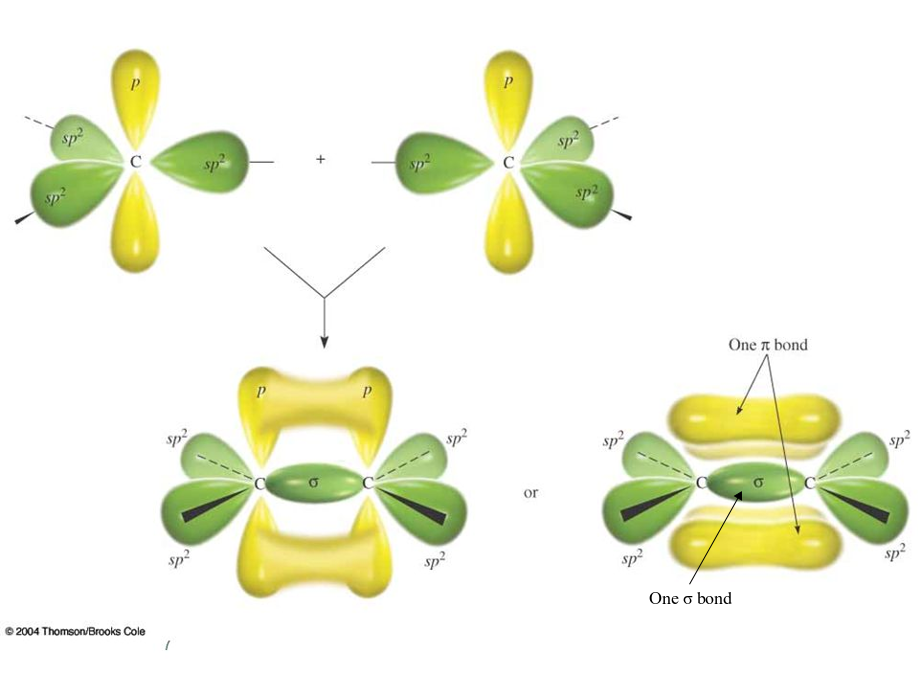
\includegraphics[width=0.7\textwidth]{double_bond}
\caption{The formation of $sp^2$ $\sigma$ and $p_z$ $\pi$ double bond. Image source: Ref. \cite{gra_bond} }  
\label{fig:gra_bond}
\end{figure} 

Every C atom has the same local environment in graphene. However, adjacent atoms are not equivalent from a symmetry point of view. They belong to different hexagonal sublattices, $A$ and $B$, as indicated with blue and yellow colors in \autoref{fig:gra_lat}. $a_1$ and $a_2$ are the basis vectors in real space connecting equivalent lattice sites. On the left, $b_1$ and $b_2$ are the basis vectors in reciprocal space connecting equivalent k points. The hexagon in reciprocal space is the first Brillouin zone where all inequivalent k points are contained. These k points correspond to different parallel lines of atoms and thus their directions in reciprocal space are associated with different directions in real space. The k wave vectors near the $\Gamma$ point have longer wave length than those away from it. While those at the boundary of the first Brillouin zone have wave lengths that are twice the unit cell dimension in the direction specified by the k points. For example, the most interesting k points for graphene are the $\mathrm{K}$ and $\mathrm{K}'$ points. These directions correspond to the $a_1$ and $a_2$ directions in real space. It is only at these k points in the Brioulloin zone that the antibonding and the bonding $\pi$ bands touch each other.  

\begin{figure}[htbp!] 
\centering  
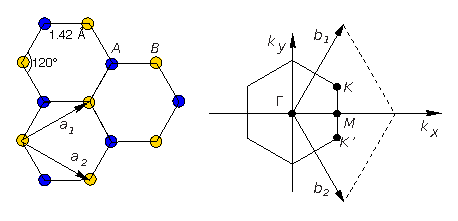
\includegraphics[width=0.8\textwidth]{gra_lat.eps}
\caption{Graphene lattice and its Brillion zone. Image source: Ref. \cite{CastroNeto2009} }  
\label{fig:gra_lat}
\end{figure} 

In contrast to $\pi$ bonds, the $\sigma$ bonds originate from a strong overlap of $sp^2$ orbitals. The interaction is so strong that the splitting of bonding and antibonding orbitals is large. This makes the $\sigma$ bonding orbitals having large negative energies, or in other words, makes the $\sigma$ bond strong and difficult to break. This feature contributes the most to the mechanical strength of graphene. On the other hand, $p_z$ orbitals are less overlapping. This makes the $\pi$ bond energy close to the Fermi level, i.e. the highest occupied state. Therefore, they contribute the most to the electronic properties of graphene.  


\subsection{Dirac cone and symmetry}

We have seen that graphene, silicene and germanene have an interesting electronic structure: forming Dirac cones. We also have listed the consequences of having such a feature: high mobility, massless carriers etc. In this section, we will discuss the symmetry condition for the existence of Dirac cones. This knowledge can be used to discover more materials exhibiting a Dirac cone. 
\begin{figure}[htbp!] 
\centering  
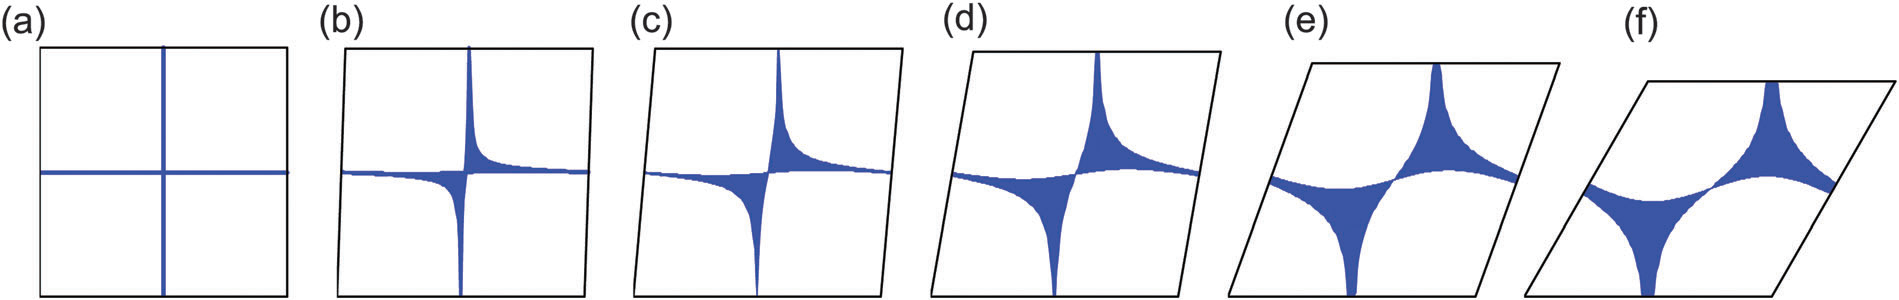
\includegraphics[width=0.95\textwidth]{dirac_hs.png}
\caption{Possible positions for the second atom (blue area) in order to guarantee the existence of Dirac cones as going from (a) square lattice to (f) hexagonal lattice. The first atom is located at the corners of the unit cell. Image source: Ref. \cite{Liu2013} }  
\label{fig:dirac_hs}
\end{figure} 
According to the von Neumann-Wigner theorem\footnote{This theorem describes the probability of a finite-dimensional matrix to has degenerated eigenvalues.}, the space-time inversion symmetry is crucial for the existence and protection of Dirac cones\cite{Wang2015b}. It is a combination of space inversion and time reversal symmetries. These two are equally important and have to act simultaneously for the possible formation of Dirac cones. A more restrictive condition that guarantees the existence of Dirac cones has to deal with relations of hopping integrals\cite{Hasegawa2006,Liu2013}. A study by \citet{Liu2013} revealed that the hexagonal lattice has the most favourable structure to form Dirac cones. The probability decreases as one goes from a hexagonal lattice to a square lattice, as shown in \autoref{fig:dirac_hs}. Therefore, since most of the 2D materials have hexagonal symmetry, there will be a higher chance of finding materials with Dirac cones in this category.

\subsection{Examples: 2D-h-BN, 2D-MoS$_2$ and graphene}
\begin{figure}[htbp!] 
\centering  
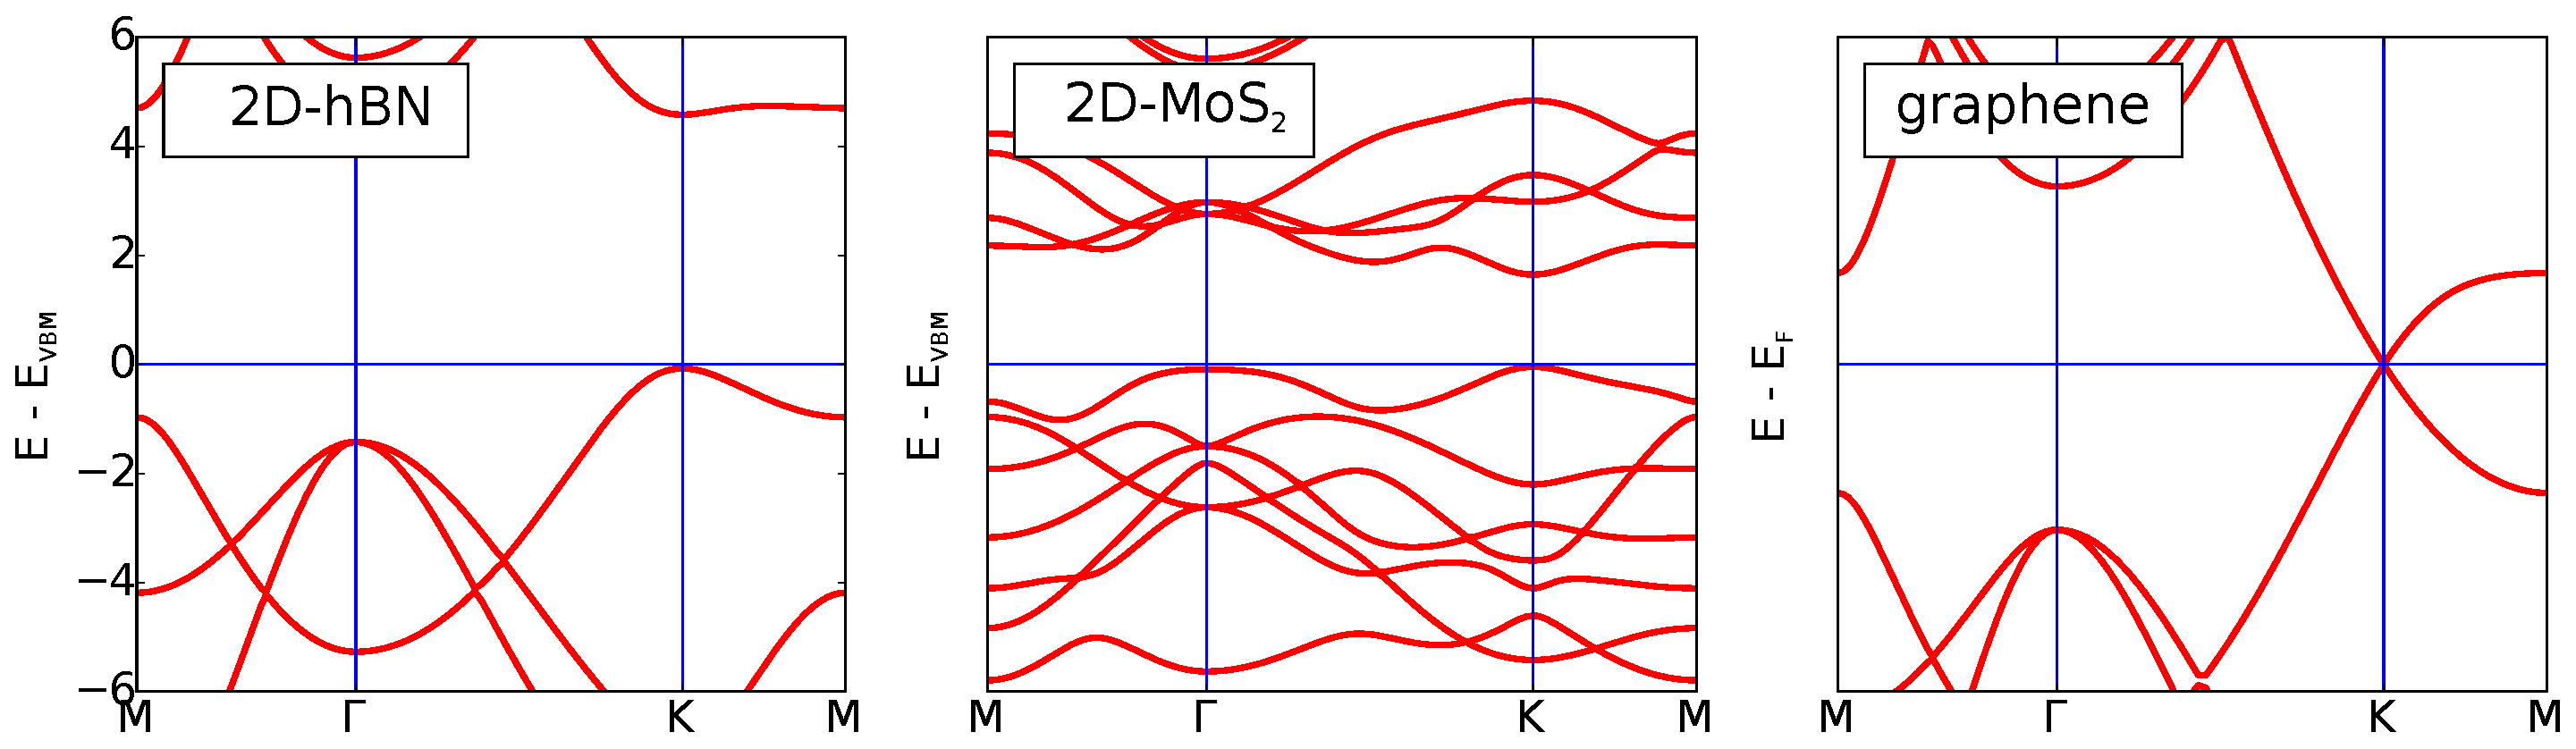
\includegraphics[width=\textwidth]{bss.eps}
\caption{Electronic band structures of 2D-hBN, 2D-MoS$_2$ and graphene calculated with PBE-GGA functional. }  
\label{fig:bss}
\end{figure} 
Three typical examples of the band structure of 2D materials are shown in \autoref{fig:bss}. The 2D h-BN is an insulator due to a large band gap in the ultraviolet range, therefore it is suitable to serve as a dielectric layer in an electronic device. The 2D TMDs have a band gap ranging from 1.0-2.5 eV which is in the visible and the near infrared range of light, therefore, they are suitable for optoelectronic device applications. Furthermore, as we compare the dispersion curves along the $\mathrm{M}\Gamma$ and $\mathrm{K}\Gamma$ directions, we can see that the electronic structure is generally the same along these paths which correspond to different crystallographic directions. This means that these materials are highly isotropic, thus we would expect the same for their physical properties. In the result chapters of this thesis, we will investigate some new 2D materials that are highly anisotropic. Their discoveries enrich the features of the physical properties of 2D materials.

\section{Vibrational properties}

The vibrational properties form an important aspect of materials, especially at finite temperature. Thermal expansion, thermal conductivity and electron mobility are all vibrational related topics. Therefore, it is crucial to understand the characterization of this in computational modelling. The force $\vec{F_I}$ on the atom $I$ at the position $\vec{R}$ can be calculated from the wave functions $\Psi_0$ evaluated from DFT thanks to the Hellmann-Feynman theorem as showing in the following: 
\begin{equation}
-\vec{F}_I=\bra{\Psi_0(\vec{R})}\nabla_I H(\vec{R})\ket{\Psi_0(\vec{R})}.
\end{equation}
When searching for the equilibrium geometry of the materials, one basically tries different positions of atoms to find a geometry that minimizes all the forces. This usually is the first thing to do for new materials, since different codes, implementations and, more importantly, different functionals will give different results. Despite the fact that the difference is usually small, an unrelaxed geometry will have residual forces on the atoms. This is particularly important when vibrational properties are concerned. Vibrational properties are characterized through the energy (usually expressed in terms of frequency) versus vibrational wave vector dispersion relation.  In crystals,  all atoms vibrate around their equilibrium positions. The vibrational modes are quantized into phonons. Each phonon represents a periodic, collective vibration with a well-defined vibrational mode and wave vector. The forces ($F$) that restore the atoms when they deviate from their equilibrium positions can be calculated from DFT either by introducing small displacements or from perturbation theory. Then, the force constants, $\Phi$, can be constructed by monitoring the change in forces through the displacements, $u$, of atoms in the following way:

\begin{equation}
\Phi_{i\alpha,j\beta}= \frac{\partial F_{j\beta}}{\partial u_{i\alpha}},
\end{equation} 
where the $i,j$ indices are the labels for atoms, $\alpha,\beta$ are the Cartesian directions: $x$, $y$ and $z$. The Fourier transformation of the force constants at wave vector $\mathbf{q}$ is the dynamical matrix $D(\mathbf{q})$ that is related to the frequency of the phonon through the eigenvalue problem:

\begin{equation}\label{eqa:w_q}
\omega^2(\mathbf{q},n)\mathbf{e}(\mathbf{q},n)=D(\mathbf{q})\mathbf{e}(\mathbf{q},n),
\end{equation}
where $\omega(\mathbf{q},n)$ is the frequency of the phonon in mode $n$ having wave vector $\mathbf{q}$, and $\mathbf{e}(\mathbf{q},n)$ is the corresponding eigenvector\cite{Ackland1997,Parlinski2011}.  Depending on whether atoms in the unit cell are vibrating in-phase or out-of-phase, phonon modes are categorized into acoustic and optical, respectively. For polar materials, charged atoms that vibrate with respect to each other can interact with light, which is the reason that these types of vibrations are called optical modes. Further, considering the respective directions of the wave ($\mathbf{e}$) and vibration ($\mathbf{q}$), the modes are subcategorized into transverse optical (TO) modes and transvers acoustice (TA) modes, where $\mathbf{q} \perp \mathbf{e}$), and longitudinal optical (LO) and longitudinal acoustic (LA) modes, where $\mathbf{q} \parallel \mathbf{e}$. These modes are all in-plane vibrations for 2D materials. For 2D materials, another direction is different from those in-plane ones, namely the $\mathbf{c}$ lattice vector direction perpendicular to the 2D plane. Special modes exist: out-of-plane transverse optical (ZO) and out-of-plane transverse acoustic (ZA) ($\mathbf{q} \perp \mathbf{e}$ and $\mathbf{q} \parallel c$). The total number of acoustic modes is three, that of optical modes is 3N-3, where N is the total number of atoms in the unit cell. 


\subsection{Example: 2D-MoS$_2$}

Let us now take layered bulk and monolayer MoS$_2$ as examples to highlight some of the important details of phonon dispersion relations. A comparison of vibrational modes between layered bulk and monolayer MoS$_2$ is presented in \autoref{fig:mos2_ph} (a). First of all, the number of atoms in the unit cell reduces from six to three from layered bulk to monolayer. Therefore, the number of optical modes will be reduced as well from 15 in layered bulk to six in the monolayer. In \autoref{fig:mos2_ph} (a) it is shown, as the material is transformed to the monolayer, that several modes merge with others that only differ by whether the vibration in different layers is in-phase or out-of-phase. Secondly, a characteristic feature of phonon disperions for layered bulk and 2D materials has appeared, namely the quadratic ZA mode (flexural mode). It is usually linear in 3D bulk materials because of strong interlayer interactions. Because in layered bulk, the interlayer interactions are weak and absent in 2D materials, therefore, it will cost less energy for the out-of-plane vibration and a quadratic dispersion will appear\cite{kittel}. This feature is closely related to the formation of the intrinsic ripples in 2D materials, e.g. graphene\cite{neek} and MoS$_2$\cite{mos2-ripple}. As shown in \autoref{fig:mos2_ph} (b), phonons with longer wave lengths, i.e. around $\Gamma$, in ZA mode have smaller frequencies or energies. This means this mode is more easily excited at low temperature and forms ripples which can be often observed in 2D materials. The formation of ripples is crucial for the stability of 2D materials at finite temperature. Lastly, in the projected DOS, the projections of mode eigenvetors to in-plane (XY) and out-of-plane (Z) components are shown. The modes with Z components, i.e. ZO$_1$, ZO$_2$ and ZA, contribute the most to the Z projections, and vice versa for the longitudinal and acoustic modes to the XY projection. 

\begin{figure}[htbp!] 
\centering  
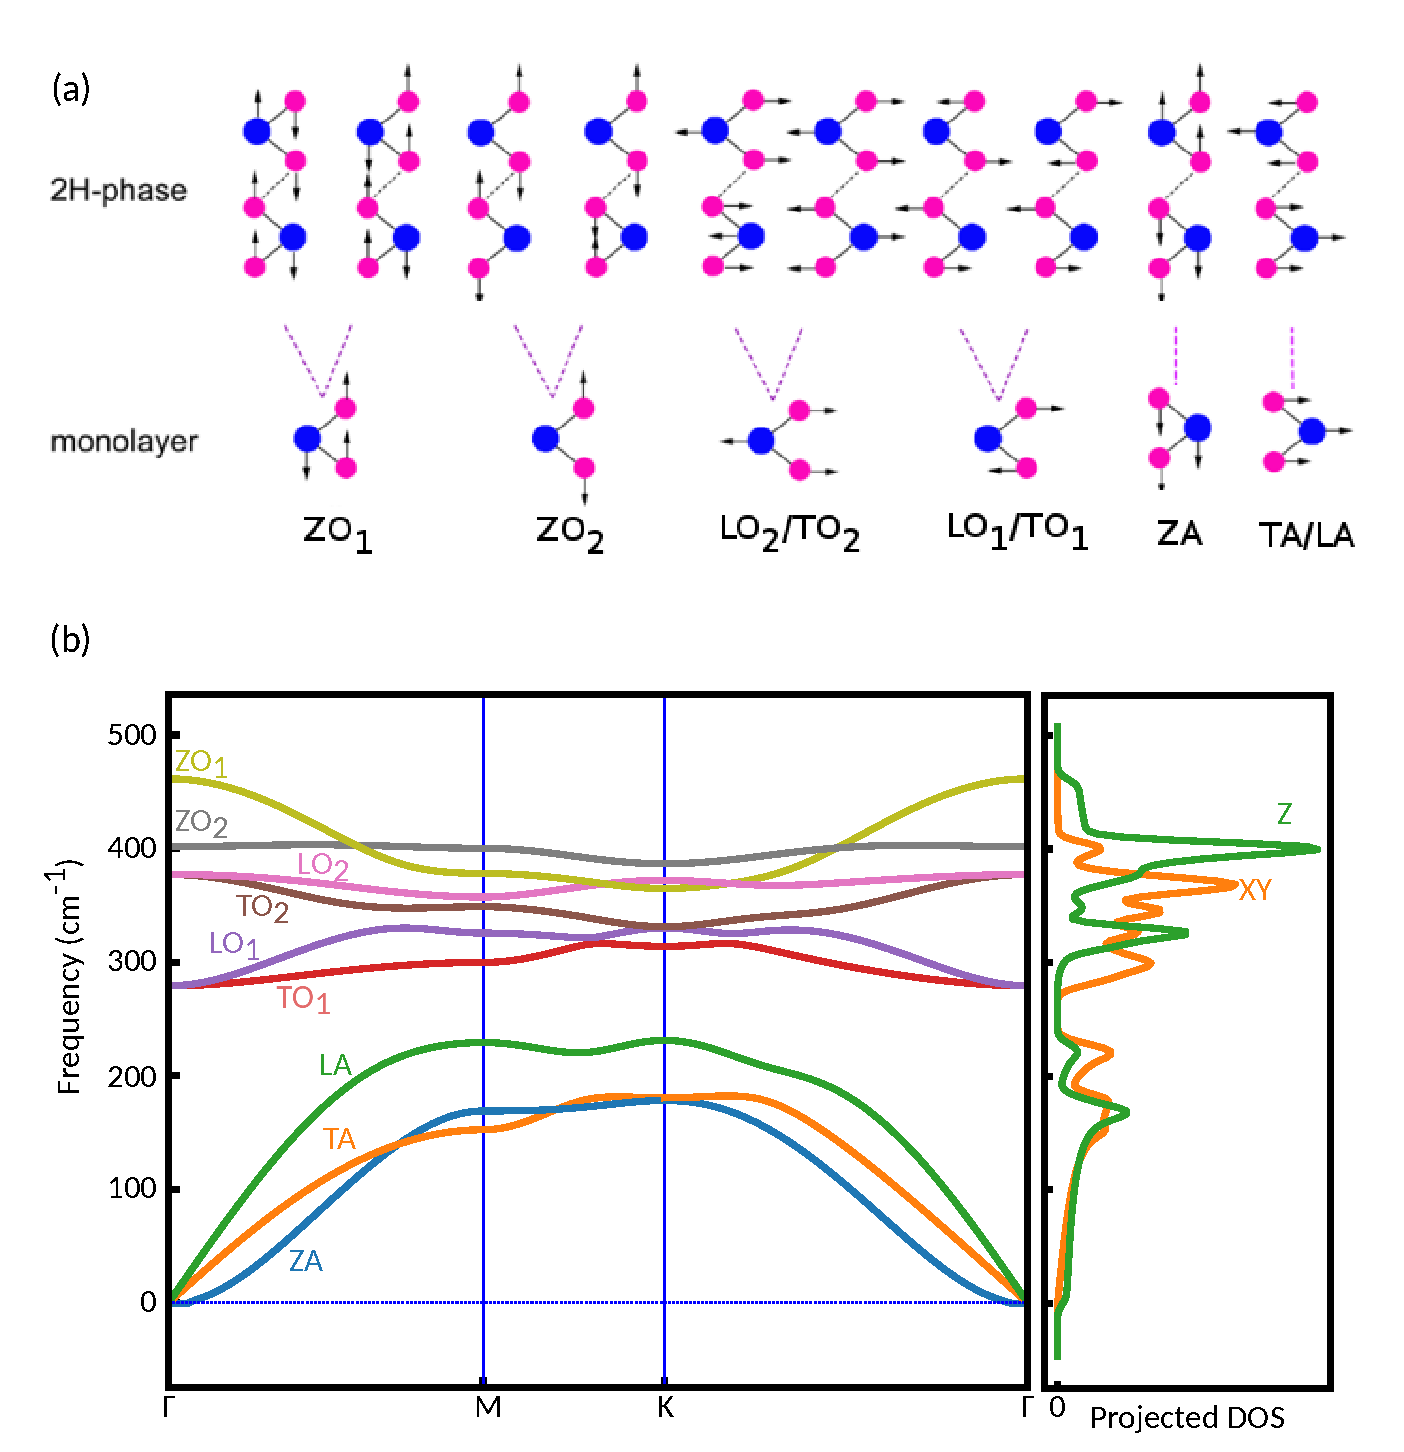
\includegraphics[width=0.8\textwidth]{ph_mos2.eps}
\caption{(a) Phonon modes of layered bulk (first row) and monolayer (second row) MoS$_2$ at the $\Gamma$ point. (b) Phonon dispersion and projected DOS of monolayer MoS$_2$.}  
\label{fig:mos2_ph}
\end{figure} 


\subsection{Dynamic stability from phonon dispersion}

One of the most useful features of the phonon dispersion is the possibility to check the dynamical stability of the structure. An unstable structure is usually indicated by the presence of imaginary frequencies in the phonon spectrum in some part of the Brillouin zone, see \autoref{fig:img_band} for example. 


\begin{figure}[htb] 
\centering  
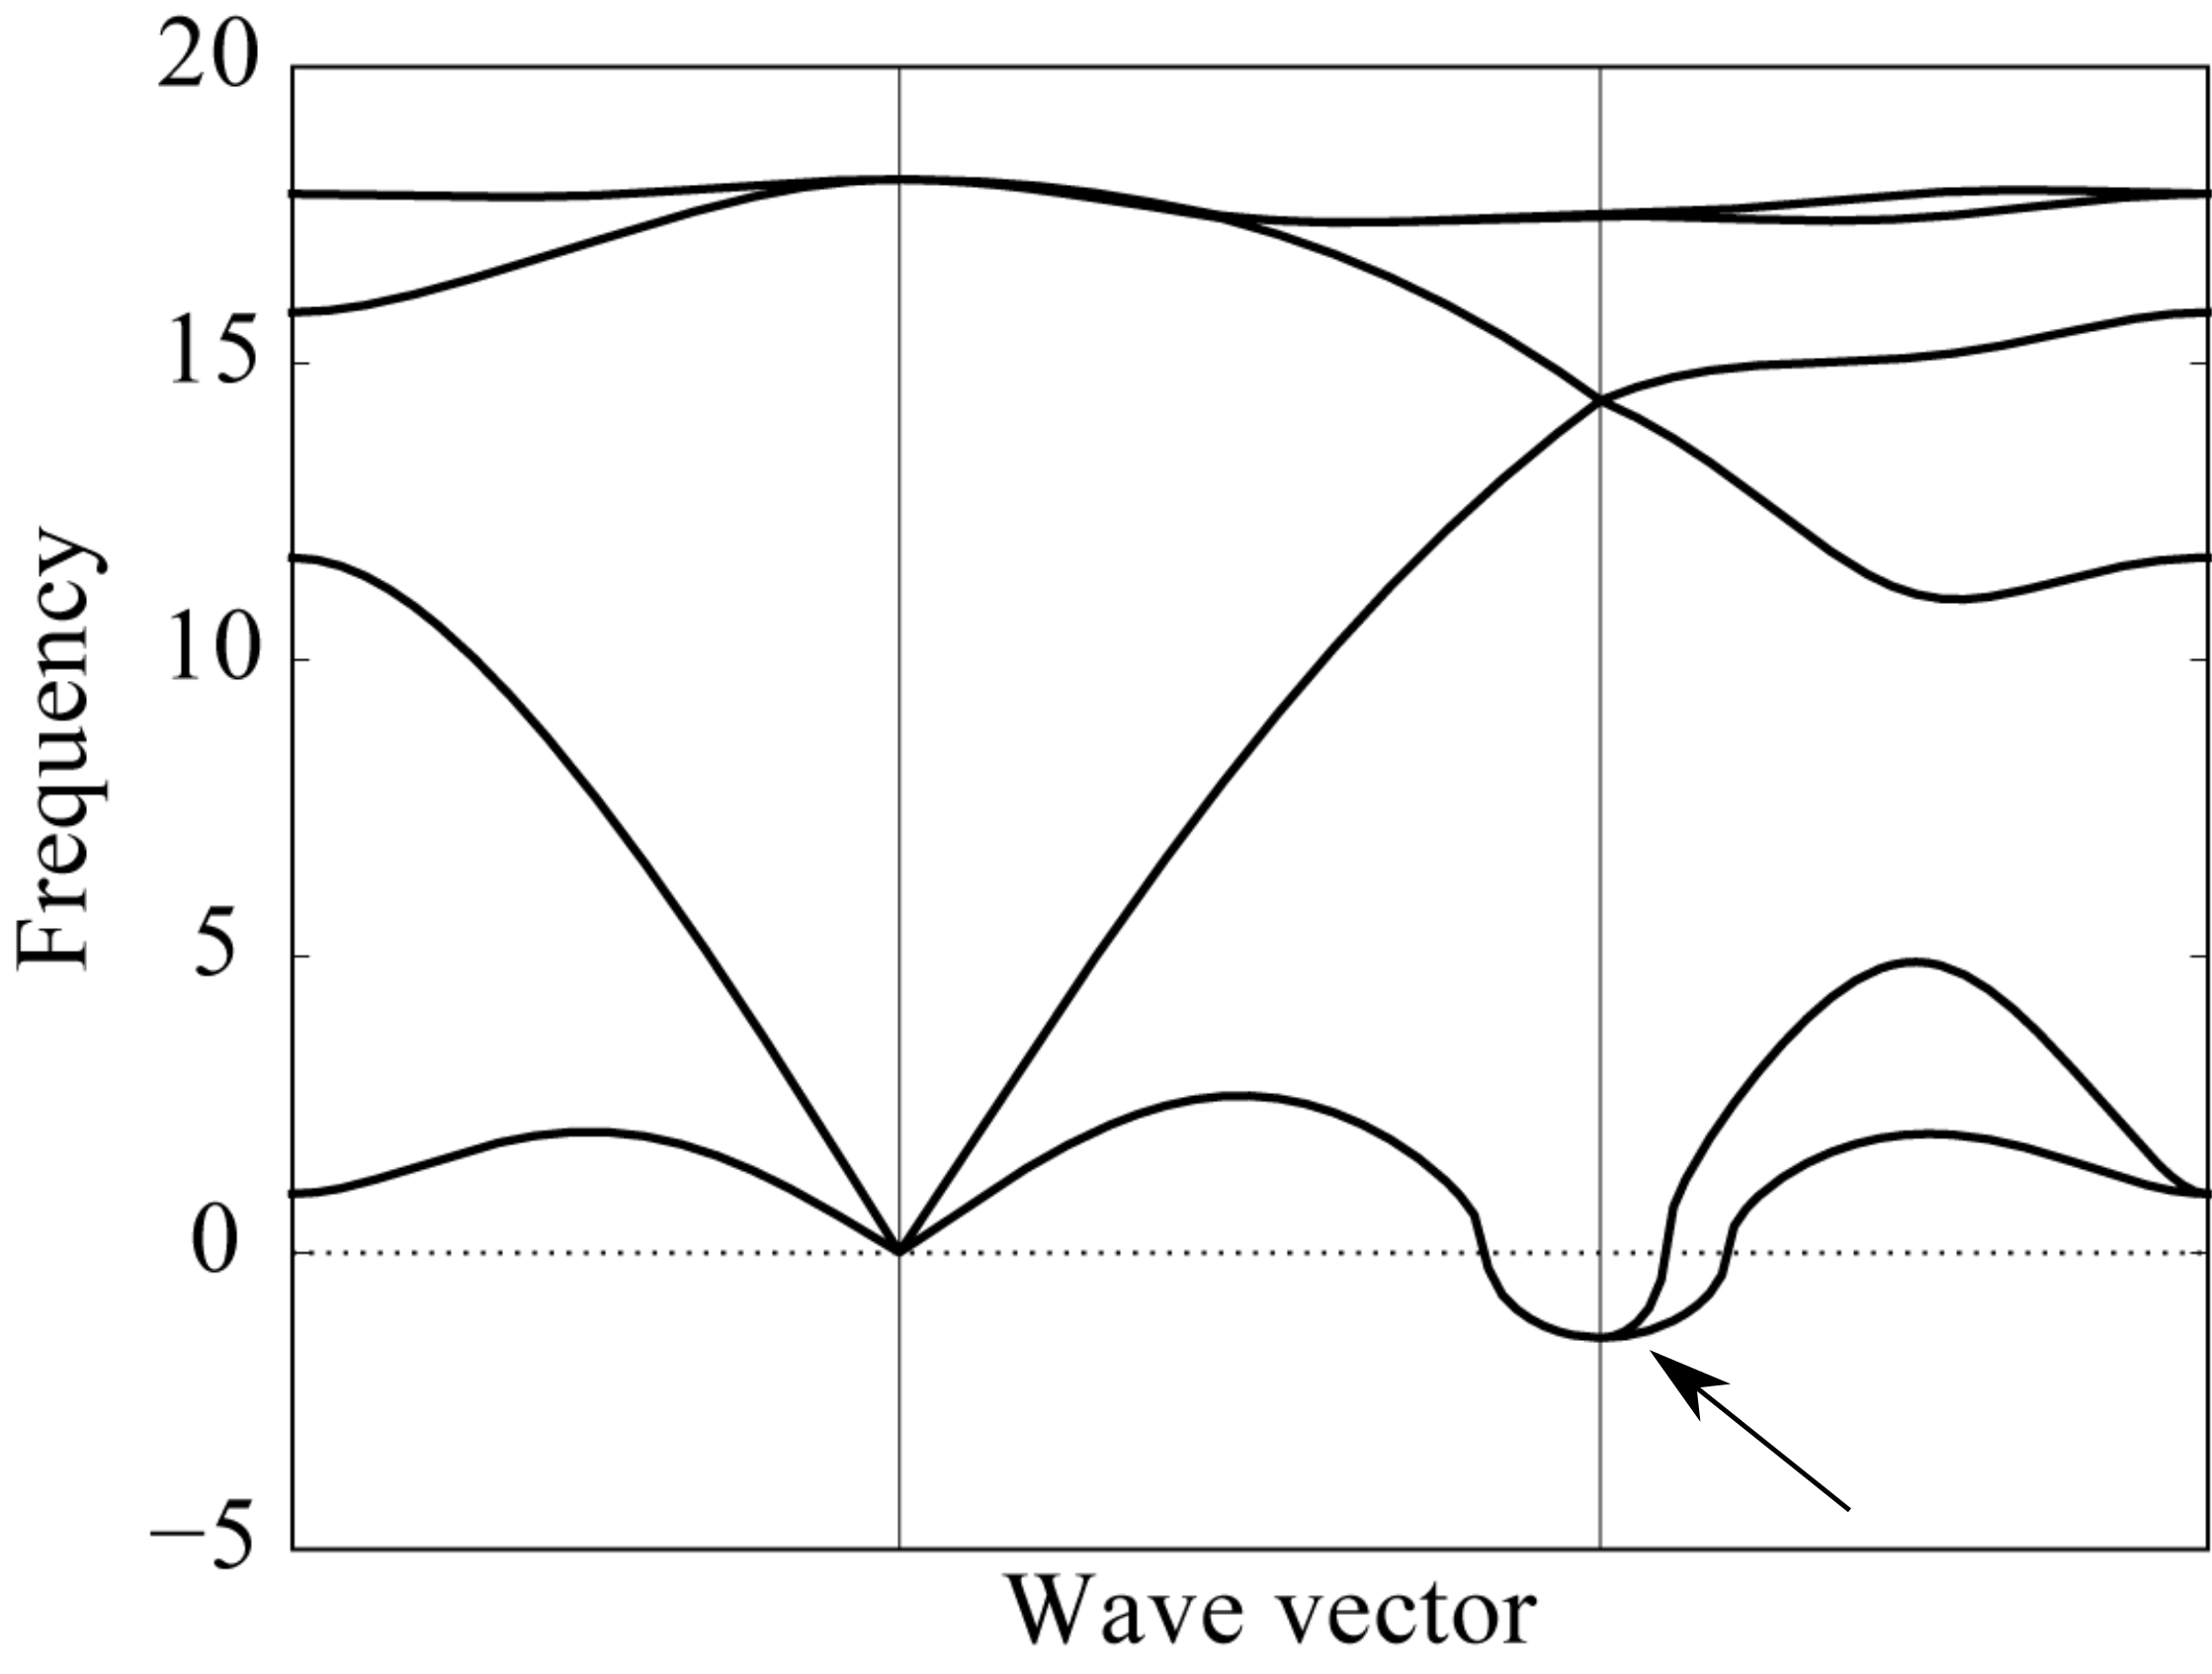
\includegraphics[width=0.5\textwidth]{img_band.png}
\caption{ Imaginary frequencies are shown as negative frequencies in a phonon dispersion plot.}  
\label{fig:img_band}
\end{figure} 

\begin{figure}[htb] 
\centering  
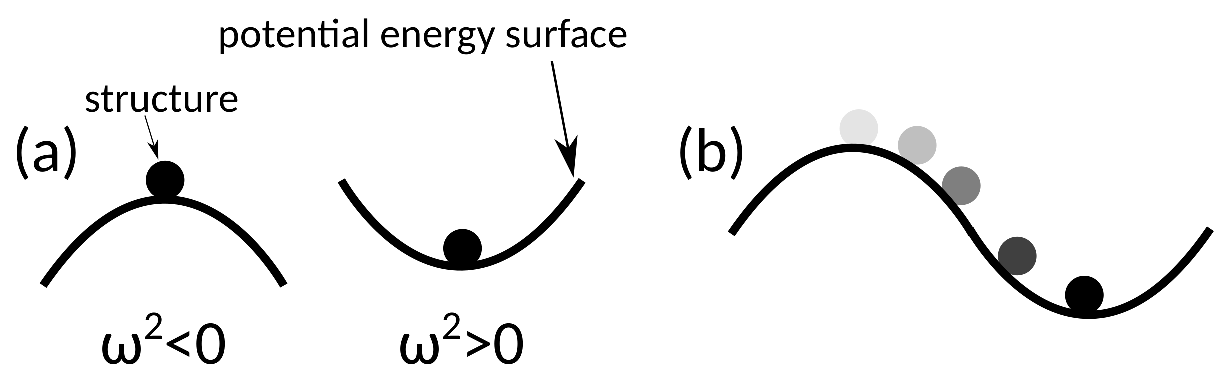
\includegraphics[width=0.7\textwidth]{fre_ima.eps}
\caption{ (a) A structure at the convex (left) and the concave (right) of the PES. (b) Searching for a stable structure (phase transition).}  
\label{fig:fre_ima}
\end{figure} 

Now let us try to understand this and make use of it to convert an unstable to a stable structure. Consider a relaxed structure in which the forces on all atoms have vanished. This could be locally at the maximum or the minimum of the potential energy surface (PES), see \autoref{fig:fre_ima}. Note that, in both situations, the forces, the derivative of the PES curves, are zero. Therefore, both situations can occur when the structure is relaxed by only following the forces. In the case of a convex PES, the dynamical matrix $D(\mathbf{q})$ will have negative components because the direction of the force is the same as the displacement. We have seen from \autoref{eqa:w_q} that $D(\mathbf{q})$ is related to the square of the frequency $\omega$, hence imaginary frequencies are the only solutions. However, a structure with imaginary frequencies near $\Gamma$ point does not necessarily mean it is not stable. Since a large supercell consisting of multiples of the unit cell is typically used to do phonon calculations, it may be that the size of the supercell is not large enough to correctly describe long wavelength phonons. In contrast to this, a structure with imaginary frequencies that appear around other q points than the $\Gamma$ point would imply a structure instability or a structural phase transition. The lowering of the energy with some vibrational modes means that the structure prefers a modulation as induced by the vibration, therefore if we calculate the energy of the modulated structure we will have a lower energy structure. With advanced techniques in phonon software\cite[e.g.][]{phonopya}, it is possible to perturb such a structure based on the vibration mode which has an imaginary frequency to find a lower energy state and stabilize the structure, as schematically illustrated in \autoref{fig:fre_ima} (b). 



\section{Mechanical properties}

In \autoref{chap:1}, we have discussed the stiffness and strength of some of the 2D materials. These are some of the mechanical properties of materials. The force on the atoms or the stress $\boldsymbol{\sigma}$ on the the unit cells under a finite strain $\boldsymbol{\epsilon}$ are typical outputs from common first-principles codes. Within the elastic regime of the stress-strain relation, they can be related through the elastic constant $\boldsymbol{C}$: $\boldsymbol{\sigma}=\boldsymbol{C}\boldsymbol{\epsilon}$, this is Hook's law. $\boldsymbol{C}$ is a 6$\times$6 matrix with matrix elements $C_{ij}$. The elements measure the resistance of a material in the $i$ direction to a deformation in the $j$ direction, where $i$ and $j$ are the index of stress and strain tensors, respectively.  With the Voigt notations, the indices have the following correspondence: 1$\rightarrow$ xx, 2$\rightarrow$ yy, 3$\rightarrow$ zz, 4$\rightarrow$ yz, 5$\rightarrow$ zx, 6$\rightarrow$ xy. The elastic constants can be simplified if the crystal symmetry and dimension are taken into account. For example, for 2D hexagonal lattice symmetry, Hook's law reads:

\begin{equation}
\begin{pmatrix} \begin{array}{c} \sigma_1 \\ \sigma_2 \\ \sigma_6 \end{array} 
\end{pmatrix}
=
 \begin{pmatrix}
  C_{11} & C_{12} & 0  \\
  C_{12} & C_{11} & 0  \\
  0 & 0 & (C_{11}-C_{12})/2
 \end{pmatrix}
 \begin{pmatrix} \begin{array}{c} \epsilon_1 \\ \epsilon_2 \\ \epsilon_6 
\end{array} \end{pmatrix}.
\end{equation} 

In this way, all elastic constants can be extracted from stress-strain data using first-principles calculations. Generally, it is more convenient to have a single quantity to describe a particular aspect of the mechanical properties of the material. This is where the Young's modulus $Y$, shear modulus $G$ and Poisson's ratio $\nu$ become useful. Following previous notations, they are defined as 

\begin{equation}
\begin{array}{c}

Y_\alpha=\frac{1}{S_{\alpha\alpha}},\hspace{6 pt} \alpha = 1, 2, 3
\end{array}.
\end{equation}

\begin{equation}
\begin{array}{c}
\nu_{\alpha\beta}=-Y_\beta S_{\alpha\beta},\hspace{6 pt} \alpha, \beta = 1, 2, 3 
\hspace{6 pt}(\alpha\neq\beta)
\end{array}.
\end{equation}

\begin{equation}
\begin{array}{c}
G_{\gamma\gamma}=\frac{1}{S_{\gamma\gamma}} ,\hspace{6 pt} \gamma = 4, 5, 6
\end{array},
\end{equation}
where $\boldsymbol{S}=\boldsymbol{C}^{-1}$ is the compliance matrix \citep[e.g.][]{nye1985physical}. The Young's modulus and shear modulus give the stiffness of the material when it responds to a stretching and shearing deformation in particular directions and they stand for the hardness of the material. Their unit in 2D is $J/m^2$ or $N/m$. To make them comparable with conventional 3D materials, 2D moduli usually are converted into 3D ones by dividing the former by the thickness of the sheet. Poisson's ratio gives the ratio of the transverse to the axial strain. It represents how easy it is to change the shape of the material with respect to changing the volume. Liquid and rubber have a Poisson's ratio close to 0.5, which is the theoretical upper limit of this quantity and making them the easiest materials to change shape over volume. In contrast, a cork has a Poisson's ratio close to zero, meaning zero lateral expansion when compressed in other directions. The breaking strength/strain is a measure of the maximum load limit that a material can withstand and it is used to characterize the strength of a material. This quantity is usually obtained by continuously deforming the material until they break and recording the maximum stress/strain. This can be done both experimentally and through simulations. 

\subsection{Examples: graphene, 2D-BN and 2D-MoS$_2$}

In \autoref{table:mech}, the mechanical properties of several 2D materials are listed, as well as that of steel for comparison.  As mentioned, graphene is the strongest material ever measured. This is due to its strong $\sigma$ bonding. With similar bonding in BN, it shows comparable results to graphene. MoS$_2$ has lower stiffness and strength than the previous two due to weaker bonding, nevertheless, it is still much stronger than steel. The Poisson's ratio has an inverse relation with Young's modulus. This means graphene acts more like cork than rubber as compared to MoS$_2$. 

\begin{table}[htb]
\caption{Mechanical properties of graphene, BN and MoS$_2$}
\centering
\label{table:mech}
\begin{tabular}{l l l l }
\hline\hline
material &   Young's modulus  & Breaking strength  &  Poisson's ratio \\
         &   TPa              & GPa               & \\
\hline
graphene\cite{Lee385} &   1.0$\pm$0.1         & 130$\pm$10               & 0.149\cite{Kudin2001} \\
2D-BN \cite{Topsakal2010}      &   0.71\textendash 0.97        & 120\textendash 165           & 0.210\\
2D-MoS$_2$\cite{Bertolazzi2011}  &   0.27$\pm$ 0.10   & 23                & 0.29 \cite{Cooper2013}\\
A36 steel\cite{steel} & 0.2 & 0.4\textendash 0.55  & 0.26 \\
\hline\hline
\end{tabular}
\end{table}

\subsection{Mechanical stability: Born stability criteria}

Mechanical stability is a criterion for unstressed crystal stability, which is additional to dynamical stability. It was first pointed out by \citet{born_1940} in the 1940’s., and is therefore often called “Born stability criteria”. Its core concept is that the elastic energy should be positive for any non-zero strains. The elastic energy $U$ is related to the elastic constants $C_{ij}$ in the following way:

\begin{equation}
U=U_0+\frac{1}{2}V_0\sum_{i,j=1}^6 C_{ij}\epsilon_i\epsilon_j,
\end{equation}
where $U_0$ is the equilibrium energy and $V_0$ is equilibrium volume. According to Born's paper\cite{born_1940}, the necessary and sufficient stability conditions are: 1) $|\mathbf{C}|>0$; 2) all eigenvalues of $\mathbf{C}$ are positive; 3) Sylvester’s criterion: the determinants of the upper-left $k$ by $k$ sub-matrices are positive; (4) an arbitrary set of minors of $\mathbf{C}$ are positive. \citet{Mouhat2014} formulated closed form expressions of this criteria for different crystal systems. Taking into account the symmetry of these systems, the number of criteria reduces, and becomes very useful to check the mechanical stability of a new crystal system. For example, for a 2D hexagonal crystal, the criteria become:

\begin{equation}
C_{11}>|C_{22}|,C_{66}>0.
\end{equation}